\documentclass[conference]{IEEEtran}
\IEEEoverridecommandlockouts

\usepackage{graphicx}
\usepackage{booktabs}
\usepackage{tabularx}
\usepackage{array}
\usepackage{amsmath}
\usepackage{xcolor}
\usepackage{tikz}
\usepackage{pgfplots}
\pgfplotsset{compat=1.17}
\usetikzlibrary{positioning,arrows.meta,calc,fit,backgrounds,shapes.geometric}
\usepackage{fontspec}
\setmainfont{TeX Gyre Termes}
\setsansfont{TeX Gyre Heros}
\setmonofont{TeX Gyre Cursor}
\usepackage{xeCJK}
% Japanese examples are quoted in the text, so a CJK face is required.
% Preference order; the first one installed wins.
\IfFontExistsTF{Noto Sans CJK JP}{\def\cjkface{Noto Sans CJK JP}}{%
  \IfFontExistsTF{Noto Sans JP}{\def\cjkface{Noto Sans JP}}{%
    \IfFontExistsTF{Yu Gothic}{\def\cjkface{Yu Gothic}}{%
      \IfFontExistsTF{MS Gothic}{\def\cjkface{MS Gothic}}{%
        \GenericError{}{No CJK font found: install Noto Sans CJK JP}{}{}}}}}
\setCJKmainfont{\cjkface}
\setCJKsansfont{\cjkface}
\setCJKmonofont{\cjkface}
\XeTeXlinebreaklocale "ja"
\XeTeXlinebreakskip=0pt plus 1pt
\usepackage{balance}
\usepackage[hidelinks]{hyperref}
\hypersetup{pdftitle={[brief] Separating Proof from Judgement in Reference-Free Evaluation of Japanese News Summaries},
            pdfauthor={Chen Jinhua}}

\definecolor{navy}{HTML}{16233A}
\definecolor{cblue}{HTML}{2563EB}
\definecolor{cbluef}{HTML}{E7EEFD}
\definecolor{cgreen}{HTML}{15803D}
\definecolor{cgreenf}{HTML}{E7F5EB}
\definecolor{corange}{HTML}{C2620A}
\definecolor{corangef}{HTML}{FDF0E0}
\definecolor{cpurple}{HTML}{6D4AA8}
\definecolor{cpurplef}{HTML}{F0EBF9}
\definecolor{cred}{HTML}{B4211C}
\definecolor{credf}{HTML}{FBECEB}
\definecolor{cgray}{HTML}{5B6B7C}

\newcolumntype{Y}{>{\raggedright\arraybackslash}X}
\newcolumntype{R}{>{\raggedleft\arraybackslash}p{9mm}}
\renewcommand{\arraystretch}{1.0}
\setlength{\tabcolsep}{3pt}

\tikzset{
  stage/.style={rounded corners=1.6pt,draw=navy,line width=.35pt,fill=white,align=left,
                inner xsep=2.2mm,inner ysep=1.5mm,font=\sffamily\fontsize{6.4}{7.4}\selectfont},
  det/.style={stage,draw=cblue,fill=cbluef},
  emb/.style={stage,draw=cgreen,fill=cgreenf},
  sem/.style={stage,draw=corange,fill=corangef},
  scr/.style={stage,draw=cpurple,fill=cpurplef},
  term/.style={stage,draw=cred,fill=credf,text=cred,align=center},
  rev/.style={draw=navy,line width=.3pt,fill=white,rounded corners=6pt,align=center,
              inner xsep=1.6mm,inner ysep=.9mm,font=\sffamily\fontsize{5.8}{6.6}\selectfont},
  fl/.style={-{Stealth[length=1.5mm,width=1.1mm]},draw=cgray,line width=.4pt},
  kill/.style={-{Stealth[length=1.5mm,width=1.1mm]},draw=cred,line width=.4pt},
  cnt/.style={font=\sffamily\fontsize{5.8}{6.6}\selectfont,text=cgray},
  ttl/.style={font=\sffamily\fontsize{6.4}{7}\selectfont\bfseries}
}

% --- A/B run naming, repeated under every table that uses it -------------
\newcommand{\tabnote}[1]{%
  \par\vspace{2.5pt}%
  \noindent\parbox{\columnwidth}{\raggedright\scriptsize #1\par}}
\newcommand{\abkey}{\textbf{A} $=$ Claude Code plugin (primary run, the
source of the submitted scores); \textbf{B} $=$ Codex plugin (secondary).}
\newcommand{\abnote}{\tabnote{\textit{Note.} \abkey}}

\title{Separating Proof from Judgement in Reference-Free Evaluation of Japanese News Summaries}

\author{\IEEEauthorblockN{Chen Jinhua}
\IEEEauthorblockA{AI Quality Scientist Take-Home Assignment\\
50 XL-Sum Japanese articles, 250 candidate summaries}}

\begin{document}
\maketitle

\begin{abstract}
A summariser in production is handed an article and returns a summary; nobody hands it a human reference. This report describes an evaluator built to that contract. Exploration showed the 250 supplied candidates are not a quality gradient but five distinct populations, and that the two most dangerous---fluent text that reverses the article, and fluent text that invents its central claim---are invisible to every cheap signal, because they are on topic by construction. The design separates constraints a script can prove from constraints only a reader can judge, and requires an independent reviewer to confirm every stopping decision. Validation rests on seven checks that do not share a failure mode, including a natural experiment in which the same candidate text appears under both its own and a foreign article, and a third independent read of the 109 candidates for which no ground truth can be derived. The evaluator ships as an installable plugin, implemented twice on two agent hosts; the two agree on routing for 94.4\,\% of candidates and on terminal category for 74 of 74.
\end{abstract}

\begin{IEEEkeywords}
LLM evaluation, reference-free metrics, summarisation quality, agent isolation, auditability, reproducibility
\end{IEEEkeywords}

\section{Exploration}

\subsection{First contact: what the 250 candidates actually are}
The dataset is 50 articles of 483--3664 characters, each with a human
reference of 41--164 and five candidates of 22--302.

Reading candidates side by side inside their articles rather than as a flat
list made the structure obvious within a few articles: the five candidates
per article are not five samples from one generator but draws from distinct
populations. A string-level scan alone---no model, no scoring---counted them
(Table~\ref{tab:census}): four are mechanically derivable, the fifth is the
remainder.

\vspace{-0.5cm}

\begin{table}[htbp]
\caption{Corpus census.}
\label{tab:census}
\vspace{-0.3cm}
\centering
\begin{tabularx}{\columnwidth}{@{}p{27mm}rY@{}}
\toprule
\textbf{Population} & \textbf{$n$} & \textbf{Derivation} \\
\midrule
Reference reproduced   & 58  & candidate $=$ reference \\
Copy of the article    & 50  & candidate $\subset$ article body \\
Reference fragment     & 17  & reference starts with candidate \\
Belongs elsewhere      & 16  & matches a \emph{different} article \\
Generated, unlabelled  & 109 & none of the above \\
\midrule
\textbf{Total}         & \textbf{250} & \\
\bottomrule
\end{tabularx}
\tabnote{\textit{Note.} Categories derived from the corpus by string
comparison alone, with no evaluator output involved; used as weak labels
only after both runs were final.}
\vspace{-0.5cm}
\end{table}

Three structural facts came out of the same scan.
\emph{The sentence limit is almost never the problem}---only three of 250
candidates exceed three sentences, and all three are article copies that
would be stopped anyway, so a rule enforcing the product specification is
necessary but will almost never fire. \emph{The corpus contains an
accidental controlled experiment}: twenty groups of candidates are
byte-identical after Unicode normalisation, eight inside a single article
and fourteen spanning two---a free reliability instrument.

\emph{The references are not ground truth, and the data says so.} The
assignment warns that XL-Sum reference quality is uneven. It is worse
than uneven: several references assert facts the article body never
contains. One reference states a 4割 sexual-assault share, a suspect
profile and a 379-case figure, none of which appear in the supplied text;
another is a photo caption opening with \mbox{この写真}, a demonstrative whose
antecedent exists only in an image nobody is given. Any design scoring a candidate by its distance to the reference
rewards it.

\subsection{Hypotheses, and which ones died}
Five hypotheses were formed before building anything. Two survived
unchanged, one survived in weakened form, and two were killed by the
data (Table~\ref{tab:hyp}).

\begin{table}[t]
\caption{Hypotheses formed during exploration and their fate.}
\label{tab:hyp}
\centering
\vspace{-0.3cm}
\begin{tabularx}{\columnwidth}{@{}>{\raggedright\arraybackslash\hyphenpenalty=10000\exhyphenpenalty=10000}p{31mm}Y@{}}
\toprule
\textbf{Hypothesis} & \textbf{Outcome} \\
\midrule
Copying is detectable with strings, not
embeddings &
\textbf{Survived.} A copy is maximally similar to its article, so
similarity is the wrong instrument; containment and $n$-gram coverage
caught 50 of 50. \\
\addlinespace[1pt]
Embedding similarity separates topic mismatch &
\textbf{Survived.} Two 10-article probes: 0.707--0.868 matched against
0.163--0.398. \\
\addlinespace[1pt]
Similarity can screen relevance on its own &
\textbf{Weakened.} On all 250 pairs the bands overlap, off-topic reaching
0.4813 and on-topic falling to 0.4034: it may nominate, not decide. \\
\addlinespace[1pt]
Missing sentence-final punctuation indicates truncation &
\textbf{Killed.} \mbox{体言止め}, a verbal noun closing a headline, is
standard news register and looks identical to an amputated predicate. \\
\addlinespace[1pt]
Factual defects form one gradient, so one faithfulness score suffices &
\textbf{Killed.} A wrong peripheral number and a reversed main event are
not two points on a scale but a flawed summary and a false one. \\
\bottomrule
\end{tabularx}
\vspace{-0.5cm}
\end{table}

The last row is the finding the design turns on. Inspecting the 109
unlabelled candidates one by one exposed a failure mode with no detector
anywhere in the pipeline as it then stood: text that is fluent,
within the sentence limit, not a copy, not truncated, on topic, and
\emph{states the opposite of the article}. One article reports the
Japanese prime minister announcing a dissolution of the lower house; its
candidate reports him announcing he will \emph{not} dissolve it. Nothing upstream can see this: the string evidence is clean and the
embedding similarity \emph{high}, because the topic is right---which is
precisely why the failure is dangerous. A sibling mode invents rather than inverts, attributing to the US
president a line, 「米国はもはや世界の警察ではない」, that appears nowhere
in the article and displaces the headline's actual claim.

Set against these, one candidate is a different animal: it substitutes
five details (シリア for イラク, 男性 for 女性, 30代 for 10代, 8000 for
6000, 500 for 300) while the central event, a fierce IS-clearing battle in
Mosul's old city, is correctly reported. It is a bad summary, not a false
one, and collapsing both into ``score zero'' throws the ranking away.

\subsection{Contributions}
These observations yield one design, implemented twice on two agent
hosts. The contributions are as follows.

\begin{enumerate}
\setlength{\itemsep}{1.5pt}

\item \emph{Data characterisation.} The 250 candidates form five distinct
populations rather than a quality gradient, only 141 of them labellable,
and the references are not ground truth. The two dominant failure modes,
reversal and fabrication, are on topic by construction, beyond any cheap
signal.

\item \emph{A stated determinism--judgement boundary.} Hard constraints
terminate and the rest is graded on a soft rubric; inside the hard tier a
script decides only what its measurement proves while a Grounding Gate
agent screens grounding before any scoring, which settles 51 of 250 pairs
deterministically and spares the most expensive stage 80 more.

\item \emph{Judge as a plugin.} Where LLM-as-a-judge is normally a
notebook and a prompt, we deliver it as an installable plugin whose role
contracts, rubric and few-shot bank are versioned files and whose records
carry a replayable trace, so a third party can run and audit the evaluator
rather than rebuild it---and, being portable, implement it twice, turning
delivery itself into a validation instrument.

\item \emph{Validation by instruments that fail differently.} The two
implementations agree with corpus-derived weak labels at 0.915 and with
each other on routing for 94.4\,\% of candidates; on the 109 candidates
carrying no derivable label a third independent reading agrees with the
submitted run at $\rho = 0.960$.

\end{enumerate}

\section{Design}

\subsection{The evidence boundary}
The runtime evaluator sees exactly one article and one candidate---never a
reference, never another article, never a corpus---because a caller who
sent one request has nothing else to give. An earlier gate ranked each
candidate against every article in the batch; it worked, and was removed
anyway, because it measured something the deployed system cannot.
References enter once, after every score is final (Section~III).

\subsection{Two layers of hard constraint, then a graded score}
Figure~\ref{fig:funnel} is the funnel, annotated with the actual counts
from the submitted run. The organising principle is that constraints
divide by what kind of evidence can settle them.

\emph{Layer~1 is physical.} Empty output, sentence count above three and
near-verbatim copying are settled by a script, because there the
measurement \emph{is} the conclusion: a containment ratio near 1.0 is not
evidence of copying, it is copying.

\emph{Layer~2 is semantic.} Whether a candidate is grounded cannot be
settled by any measurement, so a Grounding Gate agent screens every
survivor before any scoring, returning at most one central category
(\textsc{off\_topic}, \textsc{factual\_reversal},
\textsc{fabricated\_content}) with an article span and a candidate span as
evidence. It is deliberately blind to quality---no rubric, no anchor, no
score---because an agent that both screens and scores trades a central
defect for a low score.

Between the two layers sits embedding relevance, \emph{required but never
terminal}. Every survivor must leave that stage carrying a similarity
value against its own article---a run that could not reach the embedding
model is incomplete, not cheaper---but a value below threshold is only a
hint that the semantic layer should look closely.

Survivors of both layers receive a graded score
(Table~\ref{tab:rubric}). Faithfulness carries half the total because
fluent-but-false is the dominant risk here; conciseness carries five
points because the sentence limit is already a hard constraint.

\begin{table}[t]
\caption{Soft rubric.}
\label{tab:rubric}
\centering
\vspace{-0.3cm}
\begin{tabularx}{\columnwidth}{@{}p{18mm}rYr@{}}
\toprule
\textbf{Dimension} & \textbf{Max} & \textbf{Question} & \textbf{Mean} \\
\midrule
Faithfulness & 50 & Is every claim supported by the article? & 38.7 \\
Coverage     & 30 & Is the main event and its key facts present? & 19.0 \\
Coherence    & 15 & Complete, grammatical, ordered? & 13.5 \\
Conciseness  &  5 & Compact, without repetition? & 4.8 \\
\midrule
\textbf{Total} & \textbf{100} & \multicolumn{2}{r}{\textbf{76.1} over 165 survivors} \\
\bottomrule
\end{tabularx}
\tabnote{\textit{Note.} Scored only for candidates surviving both hard
layers; the four dimensions sum to the total exactly. \textbf{Mean} is
run~A (Claude Code plugin) over its 165 graded survivors.}
\vspace{-0.8cm}
\end{table}

Terminal outcomes all score 0 but keep separate rank tiers, so five
candidates remain orderable even when several fail. Reversal,
fabrication and off-topic share the worst tier, because each misleads a
reader who cannot check the source; copying and truncation rank above them.
\vspace{-0.5cm}

\begin{figure}[htbp]
\centering
\scalebox{0.85}{%
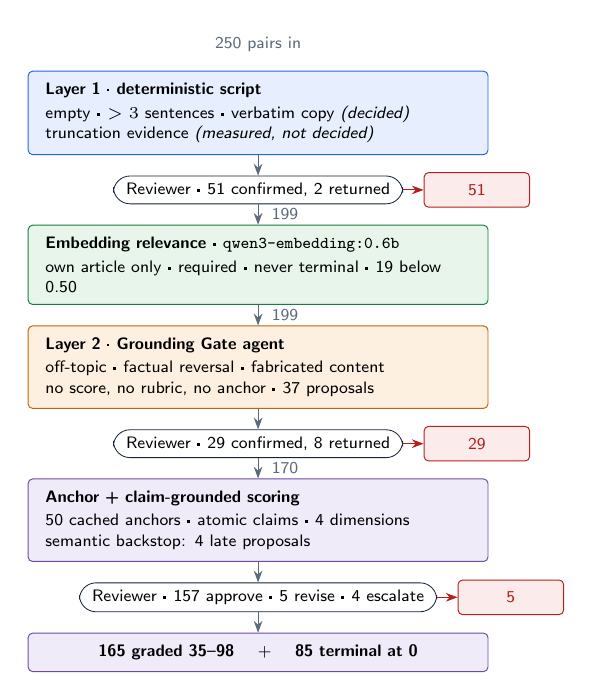
\begin{tikzpicture}[node distance=0mm]
\node[det,text width=54mm] (s1) {%
  \textbf{Layer 1 · deterministic script}\\[.4mm]
  empty · $>3$ sentences · verbatim copy \emph{(decided)}\\
  truncation evidence \emph{(measured, not decided)}};
\node[rev,below=2.6mm of s1] (r1) {Reviewer · 51 confirmed, 2 returned};
\node[emb,below=2.6mm of r1,text width=54mm] (s2) {%
  \textbf{Embedding relevance} · \texttt{qwen3-embedding:0.6b}\\[.4mm]
  own article only · required · never terminal · 19 below 0.50};
\node[sem,below=2.6mm of s2,text width=54mm] (s3) {%
  \textbf{Layer 2 · Grounding Gate agent}\\[.4mm]
  off-topic · factual reversal · fabricated content\\
  no score, no rubric, no anchor · 37 proposals};
\node[rev,below=2.6mm of s3] (r2) {Reviewer · 29 confirmed, 8 returned};
\node[scr,below=2.6mm of r2,text width=54mm] (s4) {%
  \textbf{Anchor + claim-grounded scoring}\\[.4mm]
  50 cached anchors · atomic claims · 4 dimensions\\
  semantic backstop: 4 late proposals};
\node[rev,below=2.6mm of s4] (r3) {Reviewer · 157 approve · 5 revise · 4 escalate};
\node[scr,below=2.6mm of r3,text width=54mm,align=center] (out) {%
  \textbf{165 graded 35--98} \quad + \quad \textbf{85 terminal at 0}};

\node[cnt,above=1.2mm of s1] {250 pairs in};
\coordinate (rt) at ($(s1.east)+(4.2mm,0)$);
\node[term,right=2.6mm of r1.east,yshift=0mm,text width=9mm] (t1) {51};
\node[term,right=2.6mm of r2.east,text width=9mm] (t2) {29};
\node[term,right=2.6mm of r3.east,text width=9mm] (t3) {5};

\draw[fl] (s1) -- (r1);
\draw[fl] (r1) -- node[cnt,right=0.5mm]{199} (s2);
\draw[fl] (s2) -- node[cnt,right=0.5mm]{199} (s3);
\draw[fl] (s3) -- (r2);
\draw[fl] (r2) -- node[cnt,right=0.5mm]{170} (s4);
\draw[fl] (s4) -- (r3);
\draw[fl] (r3) -- (out);
\draw[kill] (r1.east) -- (t1.west);
\draw[kill] (r2.east) -- (t2.west);
\draw[kill] (r3.east) -- (t3.west);
\end{tikzpicture}}

\caption{The funnel, annotated with counts from the submitted 250-pair
run. Red exits are Reviewer-confirmed terminations. The 51 pairs
stopped at layer~1 cost one script pass and one confirmation; 80 of 250
never reach anchor generation and scoring, the most expensive stage.}
\label{fig:funnel}
\end{figure}

\subsection{Independent review of every stopping decision}
No stage may stop a candidate on its own authority: every proposal goes to
a Reviewer in a fresh context that re-derives the evidence from the
article. It moves in both directions and is no rubber stamp: it rejected 2 of 53
physical proposals, 8 of 37 grounding proposals including all eight
fabrication claims and 3 of 4 late scorer proposals, while escalating four
truncations no gate had raised. Over-termination and missed detection are caught
by one mechanism. Disagreement surviving one round is kept
as low confidence, not averaged away.


\subsection{Alternatives considered and rejected}
Table~\ref{tab:rejected} lists the approaches tried and dropped, each with
the measurement that killed it. Two are worth naming. A cross-encoder
reranker (\texttt{bge-reranker-v2-m3}) separates off-topic text more
cleanly in mean terms but buys no recall at five times the false alarms.
And embedding the candidate against the generated anchor correlated better
with coverage yet predicted it worse under leave-one-out---a feature that
correlates better and predicts worse is fitted to the sample, so the
anchor stayed a reasoning aid and never became a number.

\vspace{-0.5cm}

\begin{table}[htbp]
\caption{Rejected approaches and the evidence that rejected them.}
\label{tab:rejected}
\centering
\vspace{-0.3cm}
\begin{tabularx}{\columnwidth}{@{}>{\raggedright\arraybackslash\hyphenpenalty=10000}p{25mm}Y@{}}
\toprule
\textbf{Approach} & \textbf{Why it was rejected} \\
\midrule
Score against the
reference &
Unavailable in production, and wrong here: generated candidates beat 45 of
50 references. \\
\addlinespace[1pt]
Similarity as a quality score &
A verbatim copy is the most similar text there is. \\
\addlinespace[1pt]
Cross-encoder reranker &
Same recall (16/16), five times the false positives (15 vs.\ 3 of 234)
at a 0.50 cut. \\
\addlinespace[1pt]
Anchor similarity as a scoring feature &
Higher correlation, worse leave-one-out error. \\
\addlinespace[1pt]
Batch-relative relevance &
Uses articles a production caller never sent; removing it changed 0 of
19 nominations. \\
\addlinespace[1pt]
Regex decides truncation &
\mbox{体言止め} is indistinguishable from an amputated predicate
without the deleted text. \\
\addlinespace[1pt]
One agent screens \emph{and} scores &
It trades a central defect for a low score instead of stopping. \\
\bottomrule
\end{tabularx}
\vspace{-0.5cm}
\end{table}

\subsection{Delivery: the design is a plugin, not a script}
The evaluator is packaged as an installable plugin, so anyone who needs it
can run it rather than reconstruct it. The primary
implementation---\textbf{run~A} below---is a Claude Code plugin carrying
four isolated agents (Grounding Gate, Scorer, Reviewer, Reporter) and the
deterministic scripts they call. There is no orchestration notebook and no
hidden state: the rubric, the few-shot bank and each agent's contract are
files under version control, so a reader can see what every role was
told.
The same design is implemented again as a Codex plugin, \textbf{run~B},
which is the instrument for the cross-host check in Section~III-E. Both
emit the same record schema, including a trace of every stage visited with
its evidence, so any score replays backwards to the measurement that
produced it.

\section{Validation}

An evaluation is worth only its weakest justification, so the goal was
several checks that fail differently rather than one repeated.
Table~\ref{tab:runs} states what the two implementations produced;
Tables~\ref{tab:pop}--\ref{tab:third} give each check's numbers.

\textbf{Naming used throughout.} \textbf{Run~A is the Claude Code
plugin}, the primary implementation and the source of the submitted
scores; \textbf{run~B is the Codex plugin}, an independent second
implementation on a different host with a different underlying model,
used as cross-host validation, never as a fallback. Every table with an A
and a B column repeats it.

\subsection{Run-level results}
Table~\ref{tab:runs} is the whole outcome of both runs; A is the submitted
one. They land on the \emph{same} count for the failure a script can
prove---50 verbatim copies---and within one for the failure an embedding
can nominate, 16 against 17 off-topic; they diverge only on the two
categories a reading must raise, A stopping 13 reversals and 1 fabrication
against B's 7 and 0. Their distributions differ in shape, not centre: B has the wider spread
and awards nearly twice as many top-band scores, so it is the more
generous reader while A stops eight more candidates. B's orchestration
also sent far more drafts back for a second round, a fact about the hosts
rather than the design; both runs end with all 250 records approved and
nothing escalated. Every disagreement below follows from it.

\vspace{-0.5cm}
\begin{table}[htbp]
\caption{Run-level results.}
\label{tab:runs}
\centering
\vspace{-0.3cm}
\resizebox{\columnwidth}{!}{%
\begin{tabular}{@{}lrr@{\hspace{3.2mm}}lrr@{}}
\toprule
 & \textbf{A} & \textbf{B} & & \textbf{A} & \textbf{B} \\
\midrule
Pairs / articles          & 250/50 & 250/50
  & \multicolumn{3}{@{}l}{\textit{Dimension mean}} \\
\multicolumn{3}{@{}l}{\textit{Routing}}
  & \quad Faithfulness \,/50 & 38.7 & 37.4 \\
Terminal                  & 85  & 77
  & \quad Coverage \,/30     & 19.0 & 20.0 \\
Graded                    & 165 & 173
  & \quad Coherence \,/15    & 13.5 & 13.9 \\
\multicolumn{3}{@{}l}{\textit{Terminal category}}
  & \quad Conciseness \,/5   & 4.8  & 4.8 \\
\quad \textsc{verbatim\_source\_copy} & 50 & 50
  & \multicolumn{3}{@{}l}{\textit{Quality label}} \\
\quad \textsc{off\_topic}      & 16 & 17
  & \quad \textsc{excellent} (90--100) & 28 & 52 \\
\quad \textsc{factual\_reversal} & 13 & 7
  & \quad \textsc{good} (75--89)       & 66 & 49 \\
\quad \textsc{obvious\_truncation} & 5 & 3
  & \quad \textsc{fine} (65--74)       & 34 & 26 \\
\quad \textsc{fabricated\_content} & 1 & 0
  & \quad \textsc{mixed} (50--64)      & 25 & 26 \\
\multicolumn{3}{@{}l}{\textit{Graded score}}
  & \quad \textsc{poor} (0--49)        & 12 & 20 \\
Mean / median             & 76.1/79 & 76.2/82
  & \multicolumn{3}{@{}l}{\textit{Review completion}} \\
SD                        & 15.1 & 19.0
  & Final decision \textsc{approve} & 250 & 250 \\
Q1 / Q3                   & 68/87 & 63/91
  & Unresolved escalations   & 0   & 0 \\
Min / max                 & 35/98 & 28/100
  & Settled in one round     & 242 & 95 \\
\multicolumn{3}{@{}l}{\textit{Record integrity}}
  & Sent back for a second   & 8   & 155 \\
Dimension-sum errors      & 0 & 0
  & Reviewer confidence \textsc{high} & 196 & 250 \\
Label-band violations     & 0 & 0 & & & \\
\bottomrule
\end{tabular}%
}

\tabnote{\textit{Note.} \abkey\ \emph{Terminal}: stopped by a confirmed
hard-constraint decision, scored 0. \emph{Graded}: reached the soft
rubric.}
\end{table}

Across all 500 records, every soft score equals the sum of its four
dimensions and every label falls inside its band: zero arithmetic errors and
zero banding violations (Table~\ref{tab:runs}).

\subsection{Determinism and a natural experiment in pair conditioning}
The corpus supplies two free instruments (Section~I-A). Eight groups of candidates are byte-identical \emph{and} attached to the
same article, each scored independently without either scorer knowing the
twin existed. All eight received identical totals and identical dimension
values in both implementations, so run-to-run variance explains none of
the spread below.

Fourteen further groups, 32 candidates, are byte-identical but split
across articles. If the evaluator graded text quality both copies would
score the same; they do not. In all 14, in both implementations, the
foreign placement was terminated at
0 as off-topic and the native placement graded on its merits---one such text scores 87
under its own article and 0 under another---the evaluator conditions on
the pair, which a text-only metric cannot.

\subsection{Agreement with corpus-derived weak labels}
After both runs were final, references were opened for the first time
and the Table~\ref{tab:census} categories were used as weak labels.
Table~\ref{tab:pop} and Fig.~\ref{fig:bands} give the per-population
outcome.
\vspace{-0.5cm}
\begin{table}[htbp]
\caption{Outcome by corpus-derived population.}
\label{tab:pop}
\centering
\vspace{-0.3cm}
\begin{tabular}{@{}lrrrrrr@{}}
\toprule
 & & \multicolumn{2}{c}{\textbf{Stop}} & \multicolumn{2}{c}{\textbf{Survivor mean}} \\
\cmidrule(lr){3-4}\cmidrule(lr){5-6}
\textbf{Population} & \textbf{$n$} & \textbf{A} & \textbf{B} & \textbf{A} & \textbf{B} \\
\midrule
Copy of the article   & 50  & 50 & 50 & ---  & ---  \\
Belongs elsewhere     & 16  & 16 & 16 & ---  & ---  \\
Reference fragment    & 17  & 5  & 3  & 59.4 & 48.4 \\
Reference reproduced  & 58  & 0  & 0  & 78.6 & 79.9 \\
Generated             & 109 & 14 & 8  & 76.6 & 77.9 \\
\midrule
\multicolumn{2}{@{}l}{Agreement, 141 labelled}
                            & \multicolumn{2}{r}{129 \,/\, 127}
                            & \multicolumn{2}{r}{0.915 \,/\, 0.901} \\
\bottomrule
\end{tabular}
\tabnote{\textit{Note.} \abkey\ \emph{Stop}: candidates terminated; the
score columns cover survivors only. \emph{Agreement}: routing matches the
population's expectation---copies, foreign placements and fragments stop,
reference reproductions do not.}
\vspace{-0.35cm}
\end{table}

Survivor ranges tell more than the means: fragments survive at 39--70 and
34--63, reference reproductions at 42--89 and 40--99, generated candidates
at 35--98 and 28--100, and no surviving fragment reaches \textsc{good}. Two things in Fig.~\ref{fig:bands} matter
more than the headline figure. The fragment population is graded rather
than uniformly stopped---a deliberate divergence from the label, discussed
in Section~IV-B---and in run~A \emph{no} reference reproduction reached
\textsc{excellent} while 28 generated candidates did, the
reference-quality problem of Section~I made quantitative. Run~B puts 10
references in the top band against 42 generated ones, so the ordering
survives.

\vspace{-0.5cm}

\begin{figure}[htbp]
\centering
\scalebox{0.85}{%
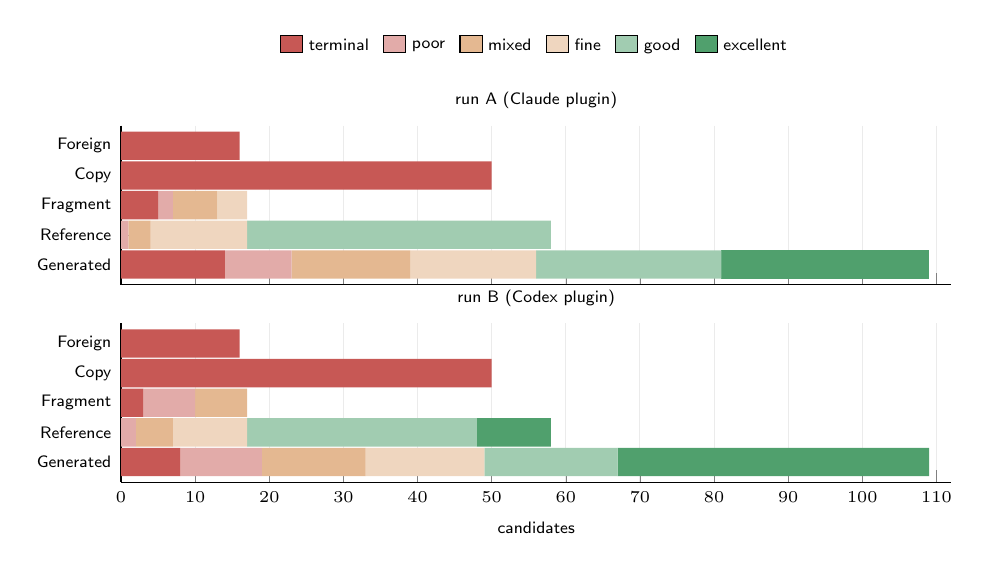
\begin{tikzpicture}
\begin{axis}[
  name=axA,
  width=\columnwidth, height=36mm,
  xbar stacked, xmin=0, xmax=112,
  bar width=3.6mm,
  ytick=data,
  symbolic y coords={Foreign,Copy,Fragment,Reference,Generated},
  y dir=reverse,
  tick label style={font=\sffamily\fontsize{5.8}{6.6}\selectfont},
  label style={font=\sffamily\fontsize{6.2}{7.2}\selectfont},
  title={\sffamily\fontsize{6.2}{7.2}\selectfont run A (Claude plugin)},
  title style={yshift=-1.2mm},
  xticklabels={},
  legend style={font=\sffamily\fontsize{5.6}{6.4}\selectfont,
                at={(0.5,1.62)},anchor=north,legend columns=6,
                draw=none,/tikz/every even column/.append style={column sep=1.1mm}},
  axis lines*=left,
  xmajorgrids, grid style={draw=black!8},
  enlarge y limits=0.17,
]
\addplot[fill=cred!75,draw=none] coordinates {(16,Foreign) (50,Copy) (5,Fragment) (0,Reference) (14,Generated)};
\addplot[fill=cred!38,draw=none] coordinates {(0,Foreign) (0,Copy) (2,Fragment) (1,Reference) (9,Generated)};
\addplot[fill=corange!45,draw=none] coordinates {(0,Foreign) (0,Copy) (6,Fragment) (3,Reference) (16,Generated)};
\addplot[fill=corange!26,draw=none] coordinates {(0,Foreign) (0,Copy) (4,Fragment) (13,Reference) (17,Generated)};
\addplot[fill=cgreen!40,draw=none] coordinates {(0,Foreign) (0,Copy) (0,Fragment) (41,Reference) (25,Generated)};
\addplot[fill=cgreen!75,draw=none] coordinates {(0,Foreign) (0,Copy) (0,Fragment) (0,Reference) (28,Generated)};
\legend{terminal,poor,mixed,fine,good,excellent}
\end{axis}
\begin{axis}[
  at={(axA.below south west)}, anchor=north west, yshift=-2.5mm,
  width=\columnwidth, height=36mm,
  xbar stacked, xmin=0, xmax=112,
  bar width=3.6mm,
  ytick=data,
  symbolic y coords={Foreign,Copy,Fragment,Reference,Generated},
  y dir=reverse,
  tick label style={font=\sffamily\fontsize{5.8}{6.6}\selectfont},
  label style={font=\sffamily\fontsize{6.2}{7.2}\selectfont},
  title={\sffamily\fontsize{6.2}{7.2}\selectfont run B (Codex plugin)},
  title style={yshift=-1.2mm},
  xlabel={candidates},
  axis lines*=left,
  xmajorgrids, grid style={draw=black!8},
  enlarge y limits=0.17,
]
\addplot[fill=cred!75,draw=none] coordinates {(16,Foreign) (50,Copy) (3,Fragment) (0,Reference) (8,Generated)};
\addplot[fill=cred!38,draw=none] coordinates {(0,Foreign) (0,Copy) (7,Fragment) (2,Reference) (11,Generated)};
\addplot[fill=corange!45,draw=none] coordinates {(0,Foreign) (0,Copy) (7,Fragment) (5,Reference) (14,Generated)};
\addplot[fill=corange!26,draw=none] coordinates {(0,Foreign) (0,Copy) (0,Fragment) (10,Reference) (16,Generated)};
\addplot[fill=cgreen!40,draw=none] coordinates {(0,Foreign) (0,Copy) (0,Fragment) (31,Reference) (18,Generated)};
\addplot[fill=cgreen!75,draw=none] coordinates {(0,Foreign) (0,Copy) (0,Fragment) (10,Reference) (42,Generated)};
\end{axis}
\end{tikzpicture}}

\caption{Outcome by corpus-derived population, both runs. The two
populations that should never survive never do, in either
implementation; the fragment population is graded rather than stopped;
and the reference population sits below the top of the generated
population in both.}
\label{fig:bands}
\end{figure}

\subsection{Within-article ordering}
The application needs candidates ordered inside an article, so ordering
was checked directly rather than inferred from scores
(Table~\ref{tab:order}). Across all 50 articles, in both runs, zero
articles placed a planted failure at or above the reference reproduction,
and the ordering is not degenerate: every article retained two to four
survivors with a wide spread between them, and the reference reproduction
sits at rank 2 in the large majority and never below rank 3. It is
consistently near the top without being treated as the ceiling, which is
what a design that distrusts its references should produce.
\vspace{-0.4cm}
\begin{table}[htbp]
\caption{Within-article behaviour over the 50 articles.}
\label{tab:order}
\centering
\vspace{-0.3cm}
\setlength{\tabcolsep}{2.4pt}
\begin{tabular}{@{}lrr@{\hspace{3.2mm}}lrr@{}}
\toprule
 & \textbf{A} & \textbf{B} & & \textbf{A} & \textbf{B} \\
\midrule
Planted failure $\geq$ ref. & 0 & 0
  & \multicolumn{3}{@{}l}{\textit{Survivors per article}} \\
\multicolumn{3}{@{}l}{\textit{Rank of the reference reproduction}}
  & \quad 2 survivors        & 4  & 3  \\
\quad rank 1 & 5  & 7   & \quad 3 survivors        & 27 & 21 \\
\quad rank 2 & 43 & 36  & \quad 4 survivors        & 19 & 26 \\
\quad rank 3 & 2  & 7   & \quad 0, 1 or 5          & 0  & 0  \\
\quad rank 4 or 5 & 0 & 0
  & \multicolumn{3}{@{}l}{\textit{Score spread among survivors}} \\
 & & & \quad median             & 26 & 32 \\
 & & & \quad min / max          & 6 / 61 & 2 / 68 \\
\bottomrule
\end{tabular}
\tabnote{\textit{Note.} \abkey\ \emph{Survivors}: candidates that reached
the soft rubric. \emph{Spread}: best minus worst survivor within one
article.}
\vspace{-0.4cm}
\end{table}

\subsection{Two implementations, two hosts}
The strongest available check on a design---as opposed to a run---is to
implement it twice and compare. The Codex plugin was written against the
same rubric but a different host and a different underlying model, and
neither implementation saw the other's output.
Table~\ref{tab:xhost} is the comparison; Fig.~\ref{fig:xhost} is the
same data as a scatter and a difference distribution.

\vspace{-0.3cm}
\begin{table}[htbp]
\caption{Cross-implementation agreement.}
\label{tab:xhost}
\centering
\resizebox{\columnwidth}{!}{%
\begin{tabular}{@{}lrr@{\hspace{2.4mm}}lrr@{}}
\toprule
 & \textbf{count} & \textbf{rate} & & \textbf{count} & \textbf{rate} \\
\midrule
\multicolumn{3}{@{}l}{\textit{Routing, $n=250$}}
  & \multicolumn{3}{@{}l}{\textit{Score, $n=162$}} \\
Agreement (both ways) & 236 & 0.944 & Spearman $\rho$ & & 0.891 \\
\quad both terminal & 74 & & Pearson $r$ & & 0.865 \\
\quad both graded & 162 & & Mean $|\Delta|$ & & 6.85 \\
\quad terminal in A only & 11 & & Mean $\Delta$ (SD) & & $-1.97$ (8.81) \\
\quad terminal in B only & 3 & & \quad $|\Delta| \leq 5$ & 86 & 0.531 \\
Terminal-category & 74 / 74 & 1.000 & \quad $|\Delta| \leq 10$ & 124 & 0.765 \\
\multicolumn{3}{@{}l}{\textit{Per dim., $n=162$: $\rho$ / mean $|\Delta|$}}
  & \quad $|\Delta| \leq 15$ & 145 & 0.895 \\
\quad Faithfulness \,/50 & \multicolumn{2}{r}{0.864 / 4.25}
  & \quad $|\Delta| \leq 20$ & 156 & 0.963 \\
\quad Coverage \,/30 & \multicolumn{2}{r}{0.882 / 2.96}
  & Label identical & 88 & 0.543 \\
\quad Coherence \,/15 & \multicolumn{2}{r}{0.635 / 0.70}
  & Label within one band & 157 & 0.969 \\
\quad Conciseness \,/5 & \multicolumn{2}{r}{0.243 / 0.25} & & & \\
\bottomrule
\end{tabular}%
}
\tabnote{\textit{Note.} \abkey\ Routing rows cover all 250 pairs, score
rows the 162 both implementations graded. $\Delta =$ A $-$ B; $\rho$ is
Spearman, $r$ is Pearson.}
\end{table}

The disagreements are one-sided and more informative than the agreements.
All 11 pairs stopped only by A are severity calls on a defect B also
found---6 reversals, 4 fragments and 1 fabrication, which B scored between
28 and 66---and the 3 stopped only by B were scored 58--71 by A. Not one is
a defect that only one implementation saw: the two disagree about where the
cliff is, not which candidates are near it, and all 14 come from the
populations needing a judgement.

The per-dimension block needs a caveat. Faithfulness and coverage, which
carry 80 of the 100 points and do the discriminating, correlate well.
Coherence and conciseness correlate far worse, yet differ by a fraction of
a point, because both runs push almost every survivor to the
ceiling---range restriction, not disagreement, and a sign that 15 and 5
points are more than these dimensions earn. Exact agreement
on the five-band label is 88 of 162, and 96.9\,\% of pairs fall within one
band: a mean absolute difference of 6.85 straddles boundaries 10 to 15 points
wide, so the bands are a convenience for a reader while the ordering is what
carries the decision.

\begin{figure}[t]
\centering
\scalebox{0.9}{%
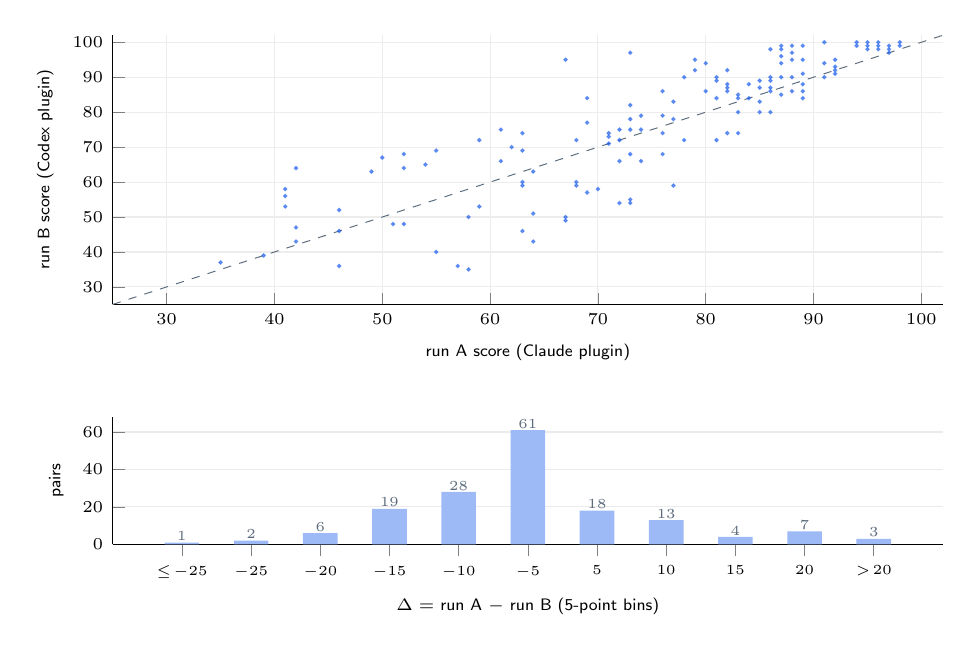
\begin{tikzpicture}
\begin{axis}[
  name=sc,
  width=\columnwidth, height=50mm,
  xmin=25,xmax=102,ymin=25,ymax=102,
  xlabel={run A score (Claude plugin)},
  ylabel={run B score (Codex plugin)},
  tick label style={font=\sffamily\fontsize{6}{7}\selectfont},
  label style={font=\sffamily\fontsize{6.4}{7.4}\selectfont},
  xtick={30,40,50,60,70,80,90,100},
  ytick={30,40,50,60,70,80,90,100},
  grid=both, grid style={draw=black!7},
  axis lines*=left,
]
\addplot[only marks,mark=*,mark size=.6pt,draw=cblue,fill=cblue,opacity=.6] coordinates {
(35,37) (39,39) (41,53) (41,56) (41,58) (42,43) (42,47) (42,64) (46,36) (46,46)
(46,52) (49,63) (50,67) (51,48) (52,48) (52,64) (52,68) (54,65) (55,40) (55,69)
(57,36) (58,35) (58,50) (59,53) (59,72) (61,66) (61,75) (62,70) (63,46) (63,59)
(63,60) (63,69) (63,74) (64,43) (64,51) (64,63) (67,49) (67,50) (67,95) (68,59)
(68,60) (68,72) (69,57) (69,77) (69,84) (70,58) (71,71) (71,73) (71,74) (72,54)
(72,66) (72,72) (72,75) (73,54) (73,55) (73,68) (73,75) (73,78) (73,82) (73,97)
(74,66) (74,75) (74,79) (76,68) (76,74) (76,79) (76,86) (77,59) (77,78) (77,83)
(78,72) (78,90) (79,92) (79,95) (80,86) (80,94) (81,72) (81,84) (81,89) (81,90)
(82,74) (82,86) (82,87) (82,88) (82,92) (83,74) (83,80) (83,84) (83,85) (84,84)
(84,88) (85,80) (85,83) (85,87) (85,89) (86,80) (86,86) (86,87) (86,89) (86,90)
(86,98) (87,85) (87,90) (87,94) (87,96) (87,98) (87,99) (88,86) (88,90) (88,95)
(88,97) (88,99) (89,84) (89,86) (89,88) (89,91) (89,95) (89,99) (91,90) (91,94)
(91,100) (92,91) (92,92) (92,93) (92,95) (94,99) (94,100) (95,98) (95,99) (95,100)
(96,98) (96,99) (96,100) (97,97) (97,98) (97,99) (98,99) (98,100)};
\addplot[draw=cgray,dashed,line width=.35pt,forget plot] coordinates {(25,25) (102,102)};
\end{axis}
\begin{axis}[
  at={(sc.below south west)}, anchor=north west, yshift=-6mm,
  width=\columnwidth, height=32mm,
  ybar, bar width=4.4mm,
  xmin=-1, xmax=11,
  ymin=0, ymax=68,
  xtick={0,1,2,3,4,5,6,7,8,9,10},
  xticklabels={$\leq\!-25$,$-25$,$-20$,$-15$,$-10$,$-5$,$5$,$10$,$15$,$20$,$>\!20$},
  x tick label style={font=\sffamily\fontsize{5.4}{6.2}\selectfont,rotate=0},
  y tick label style={font=\sffamily\fontsize{6}{7}\selectfont},
  label style={font=\sffamily\fontsize{6.4}{7.4}\selectfont},
  xlabel={$\Delta = $ run A $-$ run B (5-point bins)},
  ylabel={pairs},
  ymajorgrids, grid style={draw=black!8},
  axis lines*=left,
  nodes near coords, every node near coord/.append style=
    {font=\sffamily\fontsize{5}{5.8}\selectfont,text=cgray,yshift=-1mm},
]
\addplot[fill=cblue!45,draw=none] coordinates
  {(0,1) (1,2) (2,6) (3,19) (4,28) (5,61) (6,18) (7,13) (8,4) (9,7) (10,3)};
\end{axis}
\end{tikzpicture}}
\vspace{-0.3cm}
\caption{The 162 candidates graded by both implementations.
$\rho = 0.891$, mean $|\Delta| = 6.85$. Above: the dashed line is
equality. Below: the signed difference is centred slightly below zero
($-1.97$), the long tail is A scoring lower, and 96.3\,\% of pairs fall
within 20 points.}
\label{fig:xhost}
\end{figure}

\subsection{The block with no ground truth}
Every check so far rests on the 141 labellable candidates, the easy ones.
The 109 generated candidates---44\,\% of the corpus, and the block
carrying the fluent factual errors---have no derivable label, so reporting
0.915 while staying silent about them reports the wrong number. They were
scored a third time by a separate reading with no access to either run's
output (Table~\ref{tab:third}): on the 94 that all three readings graded
it agrees with the primary run at $\rho = 0.960$ and the secondary at
$\rho = 0.936$, both closer than the two implementations agree. Every quantity quoted in this report is
re-derived by a checker that reads only the corpus and the run outputs and
fails if any of its 199 assertions moves, so no number here need be taken on
faith.


\vspace{-0.5cm}
\begin{table}[htbp]
\caption{Third independent reading of the 109 unlabelled candidates.}
\label{tab:third}
\centering
\begin{tabular}{@{}lrrrr@{}}
\toprule
\textbf{Pair} & \textbf{$n$} & \textbf{$\rho$} & \textbf{$r$} & \textbf{mean $|\Delta|$} \\
\midrule
Third read vs.\ A & 94 & 0.960 & 0.951 & 4.09 \\
Third read vs.\ B & 94 & 0.936 & 0.924 & 5.95 \\
A vs.\ B          & 94 & 0.916 & ---   & 6.52 \\
\midrule
\textbf{Group} & \textbf{$n$} & \multicolumn{3}{r}{\textbf{third-read score}} \\
\midrule
Terminated by A   & 14 & \multicolumn{3}{r}{mean 32.5, range 20--53} \\
Terminated by B   &  8 & \multicolumn{3}{r}{mean 34.2, range 22--59} \\
Neither           & 95 & \multicolumn{3}{r}{mean 77.0} \\
\bottomrule
\end{tabular}
\tabnote{\textit{Note.} \abkey\ Upper block: the 94 candidates all three
readings graded. Lower block: candidates one run terminated, scored by a
reader not told so.}
\end{table}

The lower block of Table~\ref{tab:third} is the part that matters. A
reader who was never told which candidates had been stopped placed every
one of them at the bottom of the distribution---mean 32.5 for the 14 that
run~A terminated and 34.2 for B's 8, against 77.0 for the rest---so the
terminal decisions on the unlabelled block are corroborated by a source
that did not make them. This does not make the scores correct, since three
readings of the same rubric can share a bias and none is a human
judgement, but the signal there is reproducible.

\section{Limitations}

\subsection{What the evaluation does not measure}
No human judgement is involved, so agreement reflects reproducibility rather than correctness, and the weak-label check can itself accept a flawed reference. Beyond grammatical completeness the evaluation does not assess style, register, audience fit or newsworthiness. It asks only whether the facts a candidate selects are the article's central ones.

\subsection{What it measures poorly}
Truncation is the one place where the contract itself sets the ceiling: a
reference cut from
「…\mbox{方針を\mbox{発表}}した。」 to 「…\mbox{方針を\mbox{発表}}」 was judged
untruncated because \mbox{発表} is a verbal noun discharging the clause, and
only the deleted した。 distinguishes \mbox{体言止め} from an amputated
predicate. The fragment population therefore
splits: mid-token endings are visible and missing them is a recall problem
worth fixing, while \mbox{体言止め} endings cannot be decided from the
article and the candidate alone, so 5 of 17 charges a limit of the contract
to the detector.
The five-band labels are also less stable than the scores
(Section~III-E), and cost is uneven, since moving the truncation
judgement to the Reviewer makes a fragment consume both stages before it
is stopped.

\subsection{One structural gap, stated plainly}
The Reviewer could technically reach the corpus and its reference column, though no reference was supplied or recorded as used: a procedural safeguard, not a structural one. The next step is to re-adjudicate the 85 terminal cases with the reference-blind Reviewer and publish the delta.


\subsection{What I would do next}
More data, above everything else: the report rests on 250 pairs from 50
articles of one publisher in one language, so every threshold here---the
0.50 cut, the dimension maxima, the band boundaries---should be assumed
invalid outside that sample. The immediate work is the same funnel
over a larger Japanese corpus from several publishers, then across
languages, since constraints built on Japanese sentence segmentation and
\mbox{体言止め} register are language-specific and must be re-derived from
scratch. Only then is human adjudication of a stratified sample, and
controlled perturbation of numbers, entities, negation and causality,
worth the spend.

\section{Conclusion}
The design rests on one claim: each constraint is decided by the evidence
that settles it, and no stage stops a candidate alone.
On this corpus it held: no ordering inversion against a reference, 0.915
against the weak labels, 94.4\,\% routing agreement with an independent twin,
$\rho = 0.960$ from a third reading. And because it installs as a plugin
carrying its own trace, the next corpus is a run, not a rebuild.

\balance
\end{document}
